\documentclass{beamer}
\usetheme{Madrid}
\usecolortheme{default}
\usepackage{tikz}
\usepackage{amsmath}
\usepackage{amssymb}

\title{Introduction to Inductive Logic and Bayes Theorem}
\subtitle{Understanding Reasoning Under Uncertainty}
\author{Brendan SHea, PhD}
\date{Introduction to Logic}

\begin{document}
	
	\begin{frame}
		\titlepage
	\end{frame}
	
	\begin{frame}{Welcome to Inductive Logic: Reasoning with Uncertainty}
		\begin{itemize}
			\item In everyday life, we often must make decisions without complete information.
			\item Inductive logic provides tools to reason effectively when certainty is impossible.
			\item This course will show how to quantify and update beliefs as new evidence emerges.
			\item Learning these skills will improve your critical thinking in school and daily life.
		\end{itemize}
		
		\begin{alertblock}{Course Goals}
			\begin{itemize}
				\item Understand the foundations of inductive reasoning
				\item Master basic probability concepts
				\item Learn to apply Bayes Theorem to real-world situations
				\item Develop better decision-making skills
			\end{itemize}
		\end{alertblock}
	\end{frame}
	
	\begin{frame}{What is Inductive Logic? Making Educated Guesses}
		\begin{itemize}
			\item \textbf{Inductive logic} is reasoning that provides probable but not certain conclusions.
			\item Unlike deductive logic, inductive conclusions go beyond what's contained in the premises.
			\item We use induction whenever we learn from experience and apply it to new situations.
			\item Induction allows us to form generalizations and make predictions about the future.
		\end{itemize}
		
		\begin{center}
			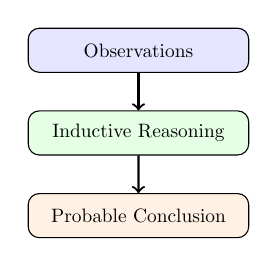
\begin{tikzpicture}[scale=0.7, transform shape]
				\node[draw, rounded corners, fill=blue!10, minimum width=4cm, minimum height=0.8cm] (obs) at (0,0) {Observations};
				\node[draw, rounded corners, fill=green!10, minimum width=4cm, minimum height=0.8cm] (ind) at (0,-1.5) {Inductive Reasoning};
				\node[draw, rounded corners, fill=orange!10, minimum width=4cm, minimum height=0.8cm] (gen) at (0,-3) {Probable Conclusion};
				
				\draw[->, thick] (obs) -- (ind);
				\draw[->, thick] (ind) -- (gen);
			\end{tikzpicture}
		\end{center}
	\end{frame}
	
	\begin{frame}{Deductive vs. Inductive Reasoning: What's the Difference?}
		\begin{itemize}
			\item \textbf{Deductive reasoning} provides conclusions that must be true if the premises are true.
			\item \textbf{Inductive reasoning} provides conclusions that are probably true, but not guaranteed.
			\item In deduction, the conclusion is contained implicitly in the premises.
			\item In induction, the conclusion goes beyond what is strictly contained in the premises.
		\end{itemize}
		
		\begin{columns}
			\begin{column}{0.48\textwidth}
				\begin{exampleblock}{Deductive Example}
					All mammals have lungs.\\
					Whales are mammals.\\
					Therefore, whales have lungs.
				\end{exampleblock}
			\end{column}
			\begin{column}{0.48\textwidth}
				\begin{exampleblock}{Inductive Example}
					Every swan I've seen is white.\\
					Therefore, probably all swans are white.\\
					(Actually false: black swans exist!)
				\end{exampleblock}
			\end{column}
		\end{columns}
	\end{frame}
	
	\begin{frame}{The Role of Probability in Inductive Reasoning}
		\begin{itemize}
			\item \textbf{Probability} is the mathematical language we use to quantify uncertainty.
			\item Inductive reasoning relies on probability to express how likely conclusions are.
			\item Probability allows us to update our beliefs as new evidence emerges.
			\item We can use probability to compare competing explanations based on available evidence.
		\end{itemize}
		
		\begin{block}{Key Question}
			Instead of asking "Is this true or false?", inductive reasoning asks "How likely is this to be true given what we know?"
		\end{block}
	\end{frame}
	
	\begin{frame}{Thinking About Probability: Frequency vs. Belief}
		\begin{itemize}
			\item There are two main ways to interpret what probability means.
			\item Each interpretation is useful in different contexts and for different problems.
			\item These interpretations lead to different approaches to statistical reasoning.
			\item Understanding both views helps us apply probability appropriately.
		\end{itemize}
		
		\begin{center}
			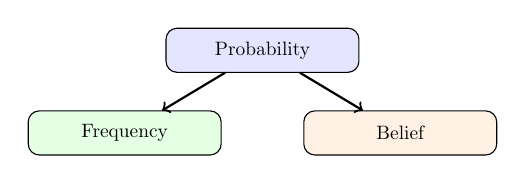
\begin{tikzpicture}[scale=0.7, transform shape]
				\node[draw, rounded corners, fill=blue!10, minimum width=3.5cm, minimum height=0.8cm] (prob) at (0,0) {Probability};
				\node[draw, rounded corners, fill=green!10, minimum width=3.5cm, minimum height=0.8cm] (freq) at (-2.5,-1.5) {Frequency};
				\node[draw, rounded corners, fill=orange!10, minimum width=3.5cm, minimum height=0.8cm] (belief) at (2.5,-1.5) {Belief};
				
				\draw[->, thick] (prob) -- (freq);
				\draw[->, thick] (prob) -- (belief);
			\end{tikzpicture}
		\end{center}
	\end{frame}
	
	\begin{frame}{Frequency-Type Probability: Counting Outcomes}
		\begin{itemize}
			\item \textbf{Frequency probability} views probability as the long-run frequency of events.
			\item It answers: "If we repeat this experiment many times, how often will this outcome occur?"
			\item This interpretation works well for events that can be repeated, like coin flips or dice rolls.
			\item Frequency probability is used in many scientific disciplines to analyze data from repeated trials.
		\end{itemize}
		
		\begin{exampleblock}{Example: Coin Flip}
			When we say a fair coin has a 50\% probability of landing heads, we mean that if we flip the coin many times, approximately half of the outcomes will be heads.
			
			$P(heads) = \frac{Number\ of\ heads}{Total\ number\ of\ flips} \approx 0.5$
		\end{exampleblock}
	\end{frame}
	
	\begin{frame}{Belief-Type Probability: Measuring Confidence}
		\begin{itemize}
			\item \textbf{Belief probability} (also called \textbf{Bayesian probability}) represents a degree of confidence.
			\item It answers: "How strongly do I believe this statement based on available evidence?"
			\item This interpretation works for one-time events that cannot be repeated, like election outcomes.
			\item Belief probability can be updated as new information becomes available.
		\end{itemize}
		
		\begin{exampleblock}{Example: Weather Forecast}
			When a meteorologist says "70\% chance of rain tomorrow," they're expressing a degree of belief based on current evidence (weather models, atmospheric conditions, etc.).
			
			$P(rain) = 0.7$ means "Based on current evidence, our confidence level in rain occurring is 70\%."
		\end{exampleblock}
	\end{frame}
	
	\begin{frame}{Basic Probability Rules: The Foundation}
		\begin{itemize}
			\item Probability is always measured between 0 (impossible) and 1 (certain).
			\item The probability of all possible outcomes for an event must sum to 1.
			\item For independent events A and B, the probability of both occurring is $P(A) \times P(B)$.
			\item For mutually exclusive events A and B, the probability of either occurring is $P(A) + P(B)$.
		\end{itemize}
		
		\begin{block}{Formula Reference}
			\begin{itemize}
				\item $P(A \text{ or } B) = P(A) + P(B) - P(A \text{ and } B)$
				\item $P(A \text{ and } B) = P(A) \times P(B)$ (if independent)
				\item $P(\text{not } A) = 1 - P(A)$
			\end{itemize}
		\end{block}
	\end{frame}
	
	\begin{frame}{Conditional Probability: When Events Affect Each Other}
		\begin{itemize}
			\item \textbf{Conditional probability} measures the likelihood of an event given another has occurred.
			\item We write this as $P(A|B)$, read as "probability of A given B."
			\item Conditional probability captures how new information changes our assessment of likelihood.
			\item This concept is fundamental to understanding Bayes Theorem.
		\end{itemize}
		
		\begin{exampleblock}{Example: Test Scores}
			Suppose 80\% of students who study pass the test, while only 30\% of students who don't study pass.
			
			$P(\text{pass}|\text{studied}) = 0.8$
			
			$P(\text{pass}|\text{didn't study}) = 0.3$
			
			The vertical bar | means "given that."
		\end{exampleblock}
	\end{frame}
	
	\begin{frame}{Introduction to Bayes Theorem: Updating What We Know}
		\begin{itemize}
			\item \textbf{Bayes Theorem} allows us to update probability estimates when new evidence emerges.
			\item It helps us move from what we knew before (prior) to what we know now (posterior).
			\item The theorem was developed by Reverend Thomas Bayes in the 18th century.
			\item Bayes Theorem has become one of the most important formulas in statistics and AI.
		\end{itemize}
		
		\begin{alertblock}{Why Bayes Theorem Matters}
			Bayes Theorem formalizes how rational people should change their minds when they encounter new information. It's the mathematical foundation for learning from experience.
		\end{alertblock}
	\end{frame}
	
	\begin{frame}{The Components of Bayes Theorem: Breaking It Down}
		\begin{itemize}
			\item Bayes Theorem involves four key components that we need to understand.
			\item These components represent different aspects of our knowledge and evidence.
			\item Understanding each component helps us apply the theorem correctly.
			\item We'll explore each component in detail over the next few slides.
		\end{itemize}
		
		\begin{center}
			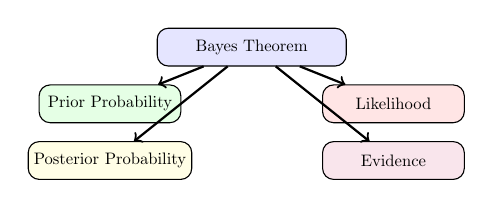
\begin{tikzpicture}[scale=0.6, transform shape]
				\node[draw, rounded corners, fill=blue!10, minimum width=4cm, minimum height=0.8cm] (bayes) at (0,0) {Bayes Theorem};
				
				\node[draw, rounded corners, fill=green!10, minimum width=3cm, minimum height=0.8cm] (prior) at (-3,-1.2) {Prior Probability};
				\node[draw, rounded corners, fill=red!10, minimum width=3cm, minimum height=0.8cm] (like) at (3,-1.2) {Likelihood};
				
				\node[draw, rounded corners, fill=yellow!10, minimum width=3cm, minimum height=0.8cm] (post) at (-3,-2.4) {Posterior Probability};
				\node[draw, rounded corners, fill=purple!10, minimum width=3cm, minimum height=0.8cm] (evid) at (3,-2.4) {Evidence};
				
				\draw[->, thick] (bayes) -- (prior);
				\draw[->, thick] (bayes) -- (like);
				\draw[->, thick] (bayes) -- (post);
				\draw[->, thick] (bayes) -- (evid);
			\end{tikzpicture}
		\end{center}
		
	\end{frame}
	
	\begin{frame}{Prior Probability: What We Believe Before Evidence}
		\begin{itemize}
			\item \textbf{Prior probability} represents our belief about an event before considering new evidence.
			\item It's written as $P(H)$, where $H$ stands for our hypothesis or claim of interest.
			\item Prior probabilities can come from previous studies, logical reasoning, or background knowledge.
			\item Even when priors are subjective, Bayes Theorem ensures that with enough evidence, different people will converge to similar conclusions.
		\end{itemize}
		
		\begin{exampleblock}{Example: Disease Diagnosis}
			If a disease affects 1 in 10,000 people in the general population, then the prior probability of having the disease is:
			
			$P(\text{disease}) = \frac{1}{10,000} = 0.0001$
			
			This is what we believe before any specific testing or symptoms are considered.
		\end{exampleblock}
	\end{frame}
	
	\begin{frame}{Likelihood: How Evidence Supports Our Hypothesis}
		\begin{itemize}
			\item \textbf{Likelihood} measures how probable the observed evidence would be if our hypothesis were true.
			\item It's written as $P(E|H)$, the probability of evidence $E$ given hypothesis $H$ is true.
			\item Likelihood is not the same as the probability of the hypothesis being true.
			\item Higher likelihood means the evidence is more consistent with our hypothesis.
		\end{itemize}
		
		\begin{exampleblock}{Example: Medical Test}
			If a test correctly identifies 95\% of people who have a disease, then:
			
			$P(\text{positive test}|\text{has disease}) = 0.95$
			
			This is the likelihood of getting a positive test result given that you have the disease.
		\end{exampleblock}
	\end{frame}
	
	\begin{frame}{Posterior Probability: Our Updated Belief}
		\begin{itemize}
			\item \textbf{Posterior probability} is our updated belief after considering the new evidence.
			\item It's written as $P(H|E)$, the probability of hypothesis $H$ given we observed evidence $E$.
			\item The posterior becomes our new prior if additional evidence becomes available later.
			\item Calculating the posterior probability is the main goal of applying Bayes Theorem.
		\end{itemize}
		
		\begin{block}{The Bayesian Learning Process}
			\begin{center}
				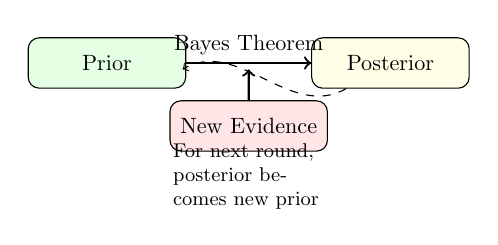
\begin{tikzpicture}[scale=0.8, transform shape]
					\node[draw, rounded corners, fill=green!10, minimum width=2.5cm, minimum height=0.8cm] (prior) at (0,0) {Prior};
					\node[draw, rounded corners, fill=yellow!10, minimum width=2.5cm, minimum height=0.8cm] (post) at (4.5,0) {Posterior};
					\node[draw, rounded corners, fill=red!10, minimum width=2.5cm, minimum height=0.8cm] (evid) at (2.25,-1) {New Evidence};
					
					\draw[->, thick] (prior) -- (post) node[midway, above] {Bayes Theorem};
					\draw[->, thick] (evid) -- (2.25,-0.1);
					
					\draw[->, dashed] (post) to[out=-150, in=30] (1.2,-0.1);
					\node[text width=2.5cm, font=\small] at (2.3,-1.8) {For next round, posterior becomes new prior};
				\end{tikzpicture}
			\end{center}
		\end{block}
	\end{frame}
	
	\begin{frame}{The Evidence Term P(E): Total Probability}
		\begin{itemize}
			\item The denominator in Bayes Theorem, $P(E)$, represents the total probability of observing our evidence.
			\item We often expand this into: $P(E) = P(E|H) \times P(H) + P(E|\neg H) \times P(\neg H)$
			\item This uses the law of total probability to consider all ways the evidence might occur.
			\item This expansion is crucial for correctly normalizing our posterior probability.
		\end{itemize}
		
		\begin{block}{Why We Decompose P(E)}
			\begin{center}
				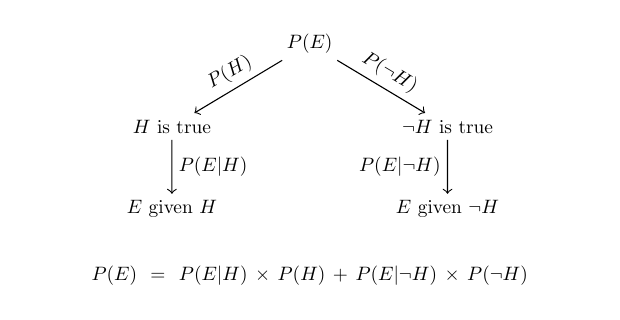
\begin{tikzpicture}[scale=0.7, transform shape]
					% Draw tree diagram
					\node (start) at (0,0) {$P(E)$};
					
					\node (h) at (-2.5,-1.5) {$H$ is true};
					\node (noth) at (2.5,-1.5) {$\neg H$ is true};
					
					\node (eh) at (-2.5,-3) {$E$ given $H$};
					\node (enoth) at (2.5,-3) {$E$ given $\neg H$};
					
					% Connections
					\draw[->] (start) -- (h) node[midway, above, sloped] {$P(H)$};
					\draw[->] (start) -- (noth) node[midway, above, sloped] {$P(\neg H)$};
					
					\draw[->] (h) -- (eh) node[midway, right] {$P(E|H)$};
					\draw[->] (noth) -- (enoth) node[midway, left] {$P(E|\neg H)$};
					
					% Final equation
					\node[text width=10cm, align=center] at (0,-4.2) {$P(E) = P(E|H) \times P(H) + P(E|\neg H) \times P(\neg H)$};
				\end{tikzpicture}
			\end{center}
		\end{block}
	\end{frame}
	
	\begin{frame}{Bayes Theorem Formula: Putting It All Together}
		\begin{itemize}
			\item Bayes Theorem combines prior probability, likelihood, and evidence to calculate posterior probability.
			\item The formula relates conditional probabilities in a powerful and elegant way.
			\item Understanding each part of the formula helps us apply it correctly to real problems.
			\item The denominator represents the total probability of observing our evidence.
		\end{itemize}
		
		\begin{alertblock}{Bayes Theorem Formula}
			\begin{center}
				$P(H|E) = \frac{P(E|H) \times P(H)}{P(E)}$
				
				\bigskip
				
				$\text{Posterior} = \frac{\text{Likelihood} \times \text{Prior}}{\text{Evidence}}$
			\end{center}
			
			Where $P(E) = P(E|H) \times P(H) + P(E|\neg H) \times P(\neg H)$
		\end{alertblock}
	\end{frame}
	
	\begin{frame}{Bayes Theorem Step-by-Step: A Simple Example}
		\begin{itemize}
			\item Let's walk through Bayes Theorem with a simple, intuitive example.
			\item Consider whether it will rain today based on observing cloudy skies.
			\item We'll identify each component of Bayes Theorem for this scenario.
			\item Following these steps will help you apply the theorem to any problem.
		\end{itemize}
		
		\begin{exampleblock}{Weather Example}
			\begin{itemize}
				\item Hypothesis ($H$): It will rain today
				\item Evidence ($E$): The sky is cloudy
				\item Prior: $P(H) = 0.3$ (30\% chance of rain based on the season)
				\item Likelihood: $P(E|H) = 0.9$ (90\% of rainy days have clouds)
				\item $P(E|\neg H) = 0.4$ (40\% of non-rainy days have clouds)
				\item $P(E) = 0.9 \times 0.3 + 0.4 \times 0.7 = 0.27 + 0.28 = 0.55$
				\item Posterior: $P(H|E) = \frac{0.9 \times 0.3}{0.55} = \frac{0.27}{0.55} \approx 0.49$
			\end{itemize}
		\end{exampleblock}
	\end{frame}
	
	\begin{frame}{Common Mistakes in Applying Bayes Theorem}
		\begin{itemize}
			\item Confusing $P(H|E)$ with $P(E|H)$ - these are very different probabilities.
			\item Forgetting to calculate the total probability of evidence $P(E)$ properly.
			\item Using incorrect prior probabilities that don't reflect background knowledge.
			\item Applying Bayes Theorem when simpler methods would work better.
		\end{itemize}
		
		\begin{alertblock}{The Prosecutor's Fallacy}
			A common error in legal contexts is focusing on $P(E|H)$ instead of $P(H|E)$.
			
			For example, saying "There's only a 1 in 10,000 chance this DNA match occurred by random chance" (which is $P(E|H)$) is not the same as saying "There's a 9,999 in 10,000 chance the defendant is guilty" (which would be $P(H|E)$).
			
			Bayes Theorem helps us avoid this error by properly accounting for the prior probability.
		\end{alertblock}
	\end{frame}
	
	\begin{frame}{Medical Testing Example: Understanding False Positives}
		\begin{itemize}
			\item Medical testing provides a clear example of how Bayes Theorem works in practice.
			\item The problem of false positives shows why understanding conditional probability is important.
			\item People often incorrectly assume a positive test means they likely have the disease.
			\item Bayes Theorem helps us calculate the true probability of disease given a positive test.
		\end{itemize}
		
		\begin{block}{Medical Test Parameters}
			Let's analyze a test for a rare disease with these characteristics:
			\begin{itemize}
				\item Disease prevalence: 1 in 10,000 people (Prior: $P(D) = 0.0001$)
				\item Test sensitivity: 99\% (Likelihood: $P(+|D) = 0.99$)
				\item Test specificity: 95\% (True negative rate: $P(-|\neg D) = 0.95$)
				\item False positive rate: 5\% ($P(+|\neg D) = 0.05$)
			\end{itemize}
		\end{block}
	\end{frame}
	
	\begin{frame}{Medical Testing Example: Calculating Real Risk}
		\begin{itemize}
			\item We want to find $P(D|+)$: the probability of having the disease given a positive test.
			\item Using Bayes Theorem helps us calculate this accurately and avoid misinterpretation.
			\item The result is often surprising to people without statistical training.
		\end{itemize}
		
		\begin{exampleblock}{Calculation}
			\tiny
			\begin{align*}
				P(D|+) &= \frac{P(+|D) \times P(D)}{P(+)} \\[0.5em]
				&= \frac{P(+|D) \times P(D)}{P(+|D) \times P(D) + P(+|\neg D) \times P(\neg D)} \\[0.5em]
				&= \frac{0.99 \times 0.0001}{0.99 \times 0.0001 + 0.05 \times 0.9999} \\[0.5em]
				&= \frac{0.000099}{0.000099 + 0.049995}
				= \frac{0.000099}{0.050094}
				\approx 0.002 = 0.2\%
			\end{align*}
			
			Despite the positive test, there's only about a 0.2\% chance of having the disease!
		\end{exampleblock}
	\end{frame}
	
	\begin{frame}{Everyday Reasoning Example: Is My Friend Angry With Me?}
		\scriptsize
		\begin{itemize}
			\item We use Bayesian reasoning informally in social situations all the time.
			\item When interpreting others' behavior, we start with prior beliefs about their feelings.
			\item New evidence (like a short text response) updates our probability estimates.
			\item Multiple possible hypotheses can be compared using Bayes Theorem.
		\end{itemize}
		
		\begin{exampleblock}{Social Situation Analysis}
			You texted your friend about hanging out, and got a brief "can't today" response.
			\begin{itemize}
				\item Hypothesis A: Friend is angry with you
				\item Hypothesis B: Friend is just busy
				\item Prior: $P(A) = 0.2$ (based on recent interactions)
				\item Likelihood: $P(\text{brief response}|A) = 0.7$, $P(\text{brief response}|B) = 0.4$
				\item Posterior: $P(A|\text{brief response}) = \frac{0.7 \times 0.2}{0.7 \times 0.2 + 0.4 \times 0.8} \approx 0.30$
			\end{itemize}
			The probability your friend is angry increased from 20\% to 30\% - higher, but still not likely.
		\end{exampleblock}
	\end{frame}
	
	\begin{frame}{Technology Example: How Spam Filters Learn}
		\begin{itemize}
			\item Email spam filters use Bayesian methods to classify incoming messages.
			\item The filter starts with prior probabilities for each word appearing in spam vs. legitimate emails.
			\item Each new email updates these probabilities based on whether you mark it as spam or not.
			\item The system continuously improves as it processes more data.
		\end{itemize}
		
		\begin{block}{Naive Bayes Classifier}
			\begin{center}
				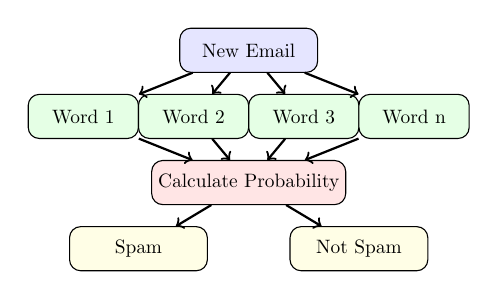
\begin{tikzpicture}[scale=0.7, transform shape]
					\node[draw, rounded corners, fill=blue!10, minimum width=2.5cm, minimum height=0.8cm] (email) at (0,0) {New Email};
					
					\node[draw, rounded corners, fill=green!10, minimum width=2cm, minimum height=0.8cm] (word1) at (-3,-1.2) {Word 1};
					\node[draw, rounded corners, fill=green!10, minimum width=2cm, minimum height=0.8cm] (word2) at (-1,-1.2) {Word 2};
					\node[draw, rounded corners, fill=green!10, minimum width=2cm, minimum height=0.8cm] (word3) at (1,-1.2) {Word 3};
					\node[draw, rounded corners, fill=green!10, minimum width=2cm, minimum height=0.8cm] (wordn) at (3,-1.2) {Word n};
					
					\node[draw, rounded corners, fill=red!10, minimum width=3.5cm, minimum height=0.8cm] (prob) at (0,-2.4) {Calculate Probability};
					
					\node[draw, rounded corners, fill=yellow!10, minimum width=2.5cm, minimum height=0.8cm] (spam) at (-2,-3.6) {Spam};
					\node[draw, rounded corners, fill=yellow!10, minimum width=2.5cm, minimum height=0.8cm] (notspam) at (2,-3.6) {Not Spam};
					
					\draw[->, thick] (email) -- (word1);
					\draw[->, thick] (email) -- (word2);
					\draw[->, thick] (email) -- (word3);
					\draw[->, thick] (email) -- (wordn);
					
					\draw[->, thick] (word1) -- (prob);
					\draw[->, thick] (word2) -- (prob);
					\draw[->, thick] (word3) -- (prob);
					\draw[->, thick] (wordn) -- (prob);
					
					\draw[->, thick] (prob) -- (spam);
					\draw[->, thick] (prob) -- (notspam);
				\end{tikzpicture}
			\end{center}
		\end{block}
	\end{frame}
	
	\begin{frame}{Philosophical Example: The Existence of God (Bayesian Perspective)}
		\begin{itemize}
			\small
			\item Philosophical arguments about God's existence can be framed in Bayesian terms.
			\item We start with a prior probability based on existing beliefs and arguments.
			\item Various pieces of evidence (like the existence of suffering) update this probability.
			\item Different people may reach different conclusions based on their priors and how they weigh evidence.
		\end{itemize}
		
		\begin{exampleblock}{A Simple Bayesian Approach}
			\scriptsize
			Consider the fine-tuning argument:
			\begin{itemize}
				\item Evidence E: The universe appears "fine-tuned" for life
				\item Hypothesis H: God exists
				\item Alternative A: Multiverse theory (many universes exist)
				\item Compare: $P(E|H)$ vs. $P(E|A)$
				\item Which hypothesis better explains the evidence?
				\item Different rational people can assess these likelihoods differently
			\end{itemize}
		\end{exampleblock}
	\end{frame}
	
	\begin{frame}{Philosophical Example: The Problem of Evil as Evidence}
		\begin{itemize}
			\item The problem of evil asks how a good, all-powerful God could allow suffering.
			\item In Bayesian terms, suffering is evidence that may affect the probability of God's existence.
			\item Theodicies (explanations for suffering) attempt to show why $P(E|H)$ is not actually low.
			\item Bayesian reasoning helps structure this debate more clearly.
		\end{itemize}
		
		\begin{columns}
			\begin{column}{0.48\textwidth}
				\scriptsize
				\begin{block}{Bayesian Problem of Evil}
					\begin{itemize}
						\item E: Suffering exists in the world
						\item H: An all-good, all-powerful God exists
						\item $P(E|H)$ seems low (unexpected)
						\item Therefore, E reduces $P(H)$
					\end{itemize}
				\end{block}
			\end{column}
			\begin{column}{0.48\textwidth}
				\scriptsize
				\begin{block}{Theodicy Response}
					\begin{itemize}
						\item Argues that $P(E|H)$ is actually not low
						\item Perhaps suffering is necessary for free will
						\item Perhaps suffering serves a higher purpose
						\item If successful, E doesn't reduce $P(H)$
					\end{itemize}
				\end{block}
			\end{column}
		\end{columns}
	\end{frame}
	
	\begin{frame}{Bayes Factor: Comparing Hypotheses}
		\begin{itemize}
			\item The \textbf{Bayes factor} is a ratio of how well two competing hypotheses predict the evidence.
			\item It's calculated as: $BF = \frac{P(E|H_1)}{P(E|H_2)}$
			\item A Bayes factor greater than 1 means the evidence supports $H_1$ over $H_2$.
			\item Bayes factors provide a way to quantify the strength of evidence.
		\end{itemize}
		
		\begin{block}{Interpreting Bayes Factors}
			\begin{center}
				\begin{tabular}{|c|l|}
					\hline
					\textbf{Bayes Factor} & \textbf{Strength of Evidence} \\
					\hline
					1 to 3 & Barely worth mentioning \\
					3 to 10 & Substantial evidence \\
					10 to 30 & Strong evidence \\
					30 to 100 & Very strong evidence \\
					$>$ 100 & Decisive evidence \\
					\hline
				\end{tabular}
			\end{center}
			
			Note: The interpretation is reversed if $BF < 1$ (evidence supports $H_2$ over $H_1$)
		\end{block}
	\end{frame}
	
	\begin{frame}{Bayesian vs. Frequentist Approaches: Two Schools of Thought}
		\begin{itemize}
			\item \textbf{Frequentist statistics} focuses on the probability of data given a hypothesis.
			\item \textbf{Bayesian statistics} focuses on the probability of a hypothesis given the data.
			\item Frequentists avoid using prior probabilities, considering only objective data.
			\item Bayesians incorporate prior information, allowing for subjective input.
		\end{itemize}
		
		\begin{columns}
			\begin{column}{0.48\textwidth}
				\scriptsize
				\begin{exampleblock}{Frequentist Approach}
					\begin{itemize}
						\item Uses p-values and confidence intervals
						\item Asks: "How likely is this data if the null hypothesis is true?"
						\item Cannot directly calculate probability of hypothesis being true
						\item Rejects or fails to reject hypotheses
					\end{itemize}
				\end{exampleblock}
			\end{column}
			\begin{column}{0.48\textwidth}
				\scriptsize
				\begin{exampleblock}{Bayesian Approach}
					\begin{itemize}
						\item Uses posterior probabilities and credible intervals
						\item Asks: "How likely is this hypothesis given the observed data?"
						\item Directly calculates probability of hypothesis
						\item Updates belief in hypotheses
					\end{itemize}
				\end{exampleblock}
			\end{column}
		\end{columns}
	\end{frame}
	
	\begin{frame}{The Power of Prior Information: Why It Matters}
		\begin{itemize}
			\item Priors allow us to incorporate existing knowledge into our analysis.
			\item They prevent us from treating each new problem as if we know nothing about it.
			\item Well-chosen priors can dramatically improve our inference, especially with limited data.
			\item As more evidence accumulates, the impact of the prior diminishes.
		\end{itemize}
		
		\begin{center}
			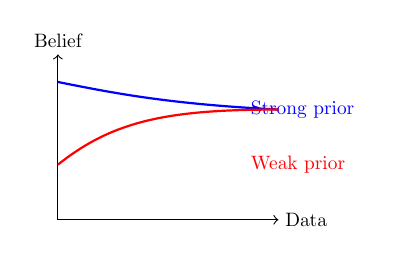
\begin{tikzpicture}[scale=0.7, transform shape]
				% Strong vs weak prior
				\begin{scope}
					\draw[->] (0,0) -- (4,0) node[right] {Data};
					\draw[->] (0,0) -- (0,3) node[above] {Belief};
					
					% Strong prior
					\draw[thick, blue] (0,2.5) .. controls (1,2.3) and (2,2.1) .. (4,2);
					\node[blue, text width=2cm] at (4.5,2) {Strong prior};
					
					% Weak prior
					\draw[thick, red] (0,1) .. controls (1,1.8) and (2,2) .. (4,2);
					\node[red, text width=2cm] at (4.5,1) {Weak prior};
				\end{scope}
			\end{tikzpicture}
		\end{center}
		
		\begin{alertblock}{Key Insight}
			\scriptsize
			With large amounts of evidence, different reasonable priors will lead to similar conclusions. However, when evidence is limited, the choice of prior can significantly affect conclusions.
		\end{alertblock}
	\end{frame}
	
	\begin{frame}{Overcoming Cognitive Biases with Bayesian Thinking}
		\begin{itemize}
			\item Human reasoning is subject to many cognitive biases that distort our judgments.
			\item Bayesian thinking provides a framework to make our reasoning more objective.
			\item It forces us to consider both prior probabilities and new evidence explicitly.
			\item Regular practice with Bayes Theorem can improve decision-making in all areas of life.
		\end{itemize}
		
		\begin{block}{Common Biases Addressed by Bayesian Thinking}
			\scriptsize
			\begin{itemize}
				\item \textbf{Base rate neglect}: Ignoring prior probabilities (corrected by using proper priors)
				\item \textbf{Confirmation bias}: Overweighting evidence that confirms existing beliefs (corrected by consistent application of Bayes Theorem to all evidence)
				\item \textbf{Availability bias}: Overestimating probabilities of easily recalled events (corrected by using data rather than anecdotes)
				\item \textbf{Anchoring}: Being unduly influenced by initial information (corrected by updating beliefs systematically)
			\end{itemize}
		\end{block}
	\end{frame}
	
	\begin{frame}{Limitations of Bayesian Reasoning}
		\begin{itemize}
			\item Bayesian methods still require good judgment in setting priors and evaluating evidence.
			\item Some situations may have too much uncertainty to provide useful probability estimates.
			\item Computational complexity can make exact Bayesian calculations difficult for complex problems.
			\item The choice of prior is sometimes controversial, especially in scientific contexts.
		\end{itemize}
		
		\begin{alertblock}{Potential Pitfalls}
			\scriptsize
			\begin{itemize}
				\item Garbage in, garbage out: Poor priors lead to poor conclusions
				\item Overconfidence: Thinking your probability estimates are more precise than they are
				\item Misapplication: Using Bayes Theorem when simpler methods would work better
				\item Complexity: Some real-world problems have too many variables for straightforward application
			\end{itemize}
		\end{alertblock}
	\end{frame}
	
	\begin{frame}{Real-World Applications: Where Bayes Theorem Is Used Today}
		\begin{itemize}
			\item Bayesian methods are increasingly important in many fields and technologies.
			\item Understanding these applications helps appreciate the power of Bayesian reasoning.
			\item The principles we've learned apply across diverse areas of research and everyday life.
			\item These applications continue to expand as computing power increases.
		\end{itemize}
		
		\begin{block}{Modern Applications of Bayesian Methods}
			\begin{columns}
				\scriptsize
				\begin{column}{0.48\textwidth}
					\begin{itemize}
						\item Machine learning and AI
						\item Medical diagnosis and testing
						\item Stock market prediction
						\item Climate science modeling
						\item Spam filtering
					\end{itemize}
				\end{column}
				\begin{column}{0.48\textwidth}
					\begin{itemize}
						\item Search engine algorithms
						\item DNA analysis and forensics
						\item Natural language processing
						\item Recommendation systems
						\item Image recognition
					\end{itemize}
				\end{column}
			\end{columns}
		\end{block}
	\end{frame}
	
	\begin{frame}{Connecting Inductive Logic to Your Life}
		\begin{itemize}
			\item Inductive reasoning and Bayesian thinking are skills you use every day, often unconsciously.
			\item Becoming more explicit about how you reason can improve decision-making.
			\item The formal tools we've learned can be applied to both academic subjects and daily life.
			\item Practice updating your beliefs based on evidence, just as Bayes Theorem prescribes.
		\end{itemize}
		
		\begin{exampleblock}{Personal Applications}
			\scriptsize
			\begin{itemize}
				\item \textbf{Education}: Evaluating which study methods are most effective for you
				\item \textbf{Social media}: Assessing the reliability of news and information
				\item \textbf{Decision-making}: Choosing between options with uncertain outcomes
				\item \textbf{Learning}: Understanding how your beliefs should change with new information
				\item \textbf{Problem-solving}: Breaking down complex issues into manageable components
			\end{itemize}
		\end{exampleblock}
	\end{frame}
	
	\begin{frame}{Conclusion: Becoming a Better Thinker with Bayes Theorem}
		\begin{itemize}
			\item Inductive logic provides tools for reasoning under uncertainty, with Bayes Theorem as a cornerstone.
			\item The Bayesian approach formalizes how rational people should update their beliefs with new evidence.
			\item These concepts apply across disciplines, from science and philosophy to everyday decision-making.
			\item By understanding probability and Bayesian reasoning, you become a more critical and effective thinker.
		\end{itemize}
		
		\begin{alertblock}{Key Takeaways}
			\scriptsize
			\begin{itemize}
				\item Uncertainty is inevitable, but we can reason rigorously within it
				\item Prior beliefs matter, but should be updated with evidence
				\item Probability is the language of inductive reasoning
				\item Bayes Theorem provides a powerful framework for learning from experience
			\end{itemize}
		\end{alertblock}
		
		\begin{center}
			\large{Questions?}
		\end{center}
	\end{frame}
	
	
\end{document}